%!TEX root = ../../main.tex
\section{A hidden Markov model of the data collection experiment}
\label{sec:A hidden Markov model of the data collection experiment}
Following the terminology in the literature the data collection experiment can be viewed as a time series: a sequence of diffraction data generated by a time-dependent process.
Time series analysis seeks to understand the underlying processes that produced the data and allow forecasting or monitoring of the process.
A more accurate analogy for the data collection experiment would be to describe it as a dose series because the changes in the crystal state (and hence the observed data) are generally attributed to a dose dependent process.

Figure~\ref{fig:Hidden Markov Model diagram} shows a schematic of the dose series model of the experiment.
At time t = i - 1 the crystal is in its initial state where the atoms have relatively well defined positions.
After an initial X-ray exposure the crystal state has changed at time t = i.
The atomic positions have changed and they have an effective smearing of their position due to an increased B-factor.
It is this state of the crystal that gives rise to the diffraction pattern at time t = i.
The process repeats itself at time t = i + 1 and beyond.
So each diffraction image can be regarded as being generated from a different but related crystal.
In the model the only components that are observed are the diffraction patterns, despite the fact that the crystal states are the desired quantities.
The crystal states are effectively `hidden`.
Furthermore the changes in crystal state as a result of X-ray exposure is assumed a Markovian process i.e. the state of the crystal at time i is completely determined by the state of the crystal at time i - 1.
The model described here is known as a hidden Markov model.
\begin{figure}[ht!]
    \centering
    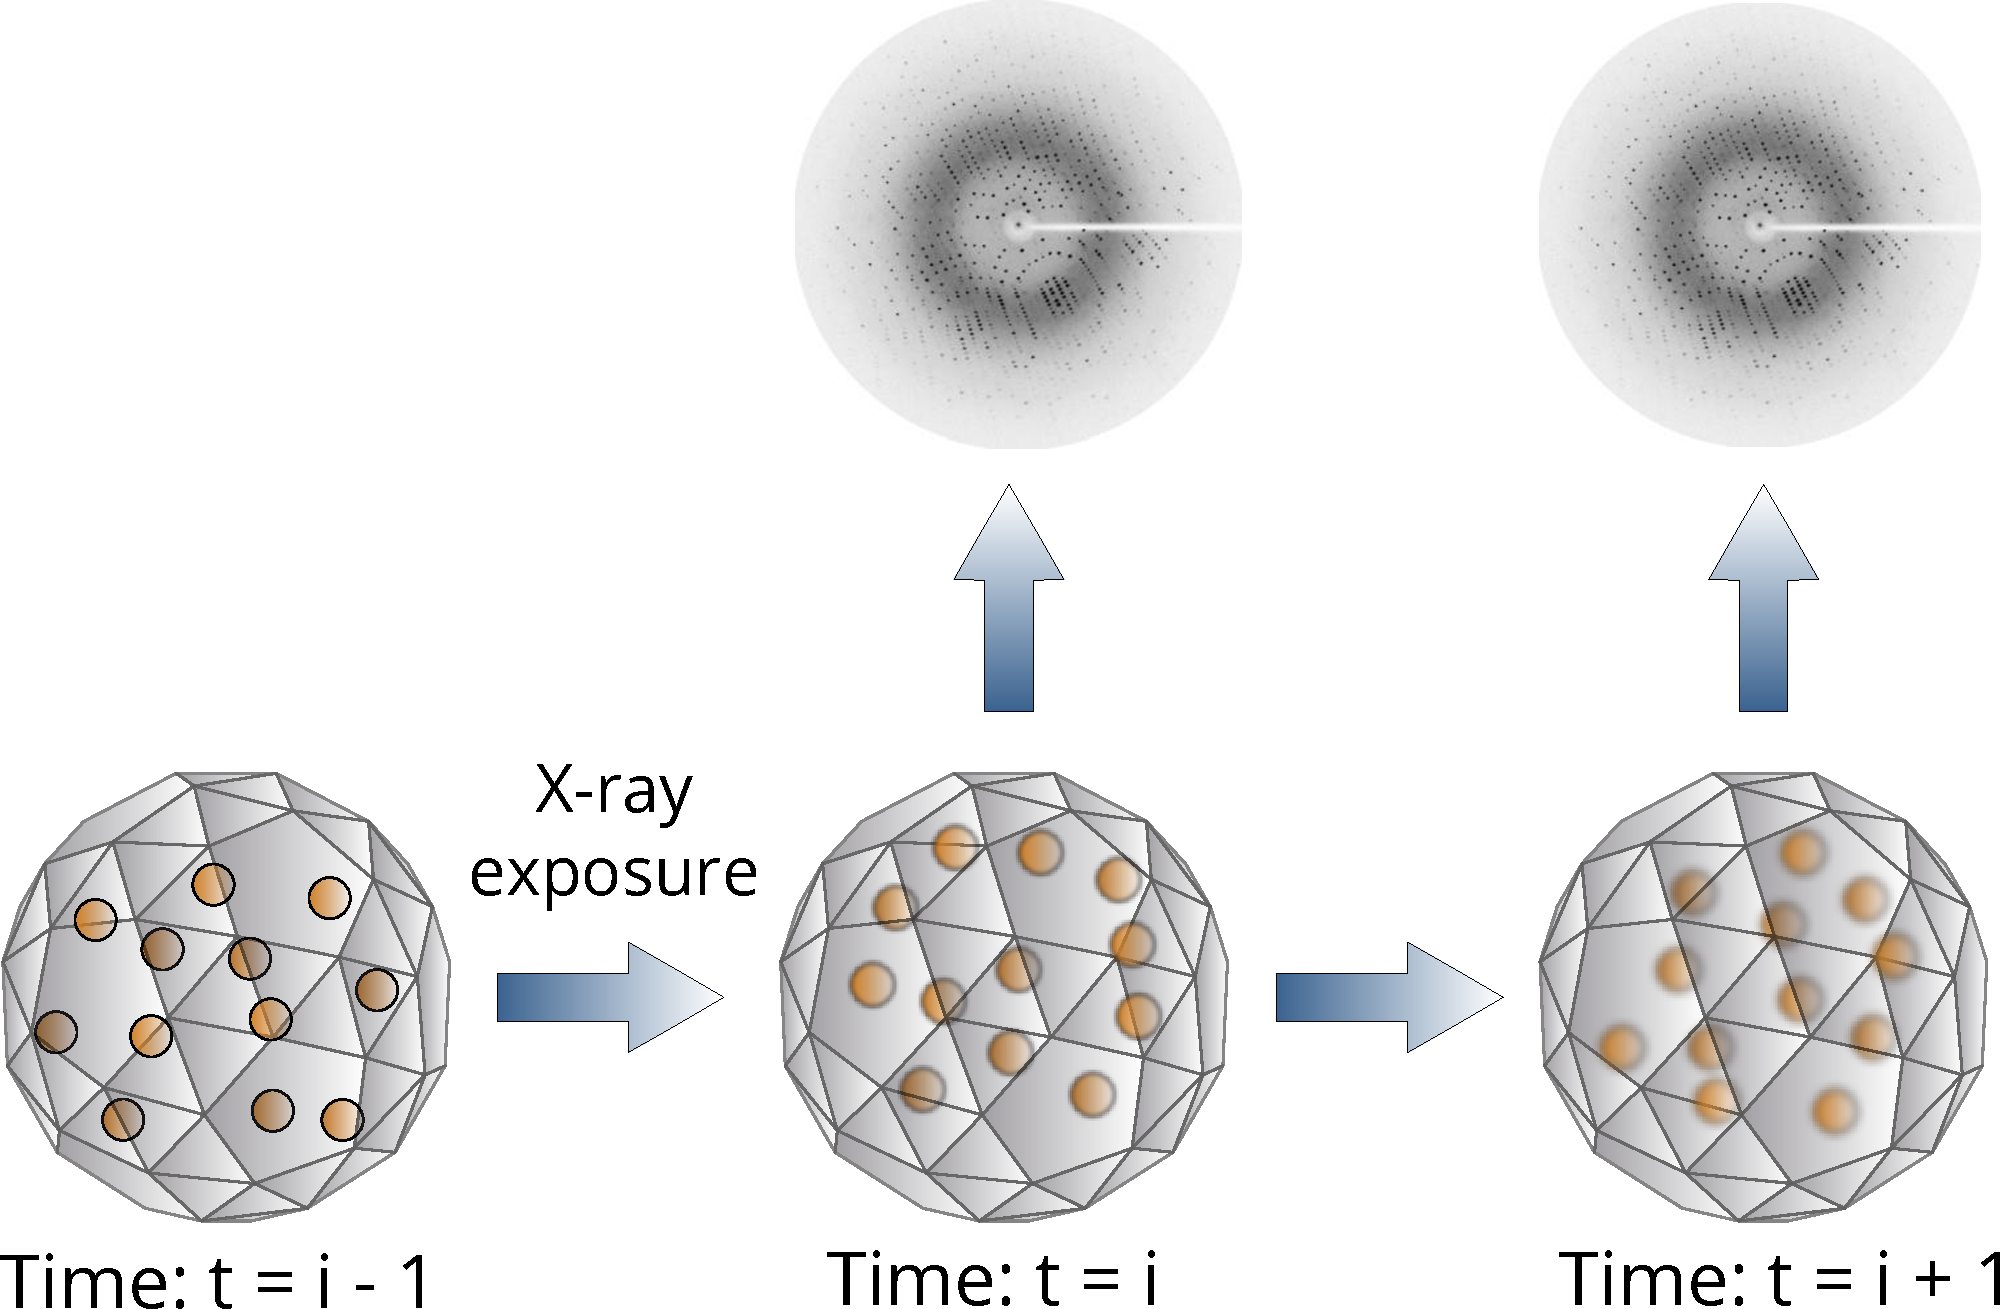
\includegraphics[width=1.0\textwidth]{figures/datared/HiddenMarkovModelDiagram.pdf}
    \caption{Hidden Markov model of the diffraction experiment.
    At time t = i - 1 the crystal is in an undamaged state and the constituent atoms have well defined positions.
    After an X-ray exposure the crystal changes state at time t = i.
    The constituent atoms change positions and their B factors increase, which is represented by a slight blurring of the atoms.
    However the state of the crystal is not observed by the experimenter, instead the experimenter observes the diffraction image that is generated as a result of the exposure.
    This process repeats itself typically until enough images have been collected to solve the structure.}
    \label{fig:Hidden Markov Model diagram}
\end{figure}

The problem can now be stated as:
\textbf{What is the most likely sequence of crystal states that generated the sequence of observed diffraction patterns?}

Before addressing the question it is necessary to understand what is meant by the crystal state.
The state of the crystal is defined by its constituent atoms and their positions.
Equivalently the state of the crystal can be described by the set of structure factors in reciprocal space: amplitudes and their corresponding phases.
However, at the data reduction stage of the crystallographic structure solution pipeline the phases are completely unknown.
Therefore the state of the crystal will be represented solely by the set of structure factor amplitudes.

\subsection{Bayesian optimal filtering}
\label{sub:Bayesian optimal filtering}
Methods used to estimate the (hidden) state, $\bs{x}_j$, of a time-varying system observed indirectly via noisy measurements, $\bs{y}_j$, at a given point in time, $j$,  are known as \textit{optimal filtering} methods.
The filtering distribution can be defined mathematically as
\begin{equation}
    P(\bs{x}_j | \bs{y}_1, \ldots, \bs{y}_j),
    \label{eq:Filtering Distribution}
\end{equation}
i.e. the probability distribution of the state given all of the previous observations up to time point $j$.
Filtering is sometimes regarded as a \textit{forwards pass} through the data.
There are many ways to define what is meant by \textit{optimal} \cite{chen2003bayesian}, here the optimality criterion is the minimum mean-squared error (MMSE) estimate of the state of the system.
Bayesian filtering refers to the formulation of an optimal filter within a Bayesian framework.
A Bayesian optimal filter can therefore be used to solve the problem of determining the crystal states given a set of (noisy) diffraction images.
Due to the non-linear relationship between the reflection intensities and the structure factor amplitudes, it is necessary to use a non-linear Bayesian optimal filter for the crystallographic diffraction experiment problem.
The filter chosen is the Unscented Kalman filter (UKF) because it propagates the probability density function in an effective manner (using the unscented transform) to achieve up to third order accuracy in the posterior mean and covariance estimates \cite{wan2000unscented}.
The UKF algorithm is outlined in \cite{wan2002Unscented}.

\subsection{Bayesian Smoothing}
\label{sub:Bayesian Smoothing}
Bayesian Smoothing can be considered to be a class of methods within the field of Bayesian filtering.
Whereas filters generally compute estimates of the system state based on the observation history, smoothers use all of the information and thus they can estimate states that happened before the current time \cite{sarkka2013}.
Mathematically the smoothing distribution is
\begin{equation}
    P(\bs{x}_j | \bs{y}_1, \ldots, \bs{y}_j, \ldots, \bs{y}_{\tau})
    \label{eq:Smoothing Distribution}
\end{equation}
where $j < \tau$.
Smoothers are regarded as \textit{backwards passes} because they can be used to estimate states prior to the current time.

The goal of the data reduction stage in the structure solution pipeline is to reduce the intensity values to accurate estimates of the structure factor amplitude for each reflection.
If this problem is phrased in a probabilistic manner then the distribution of interest is
\begin{equation}
    P(\{|\bs{F}|\}_i \,|\, \{O\}_1, \ldots, \{O\}_i,\ldots, \{O\}_{\tau}),
    \label{eq:Goal of structure determination}
\end{equation}
where $\{|\bs{F}|\}_i$ is the set of structure factor amplitudes and $\{O\}_i$ is the set of intensity measurements, $I_{hkl}$ at time point $i$.
Equation \ref{eq:Goal of structure determination} is the probability distribution that describes the values of the set of structure factor amplitudes given all of the observed data on the diffraction images.
Comparison of equations \ref{eq:Goal of structure determination} and \ref{eq:Smoothing Distribution} show that they are identical and hence using a Bayesian smoother (after application of the UKF) should provide the desired solution to the data reduction problem.
The application of both the forwards and backwards passes is known as the \textit{forward-backward algorithm}.
The important difference with this formulation compared to the current data reduction methods is that the set of structure factor amplitudes is found for every time point, $i$, as opposed to just producing a single set of amplitudes.

The Bayesian smoother chosen for this problem is the unscented Rauch-Tung-Striebel smoother (URTSS).
The algorithm for this smoother is outlined in \cite{sarkka2008unscented}.

\subsection{Process Function and covariance}
\label{sub:Process Function and covariance}
In order to apply the UKF it is necessary to define the function that relates the crystal state a time point i to the crystal state at time point i + 1.
This function is known as the process function and is typically taken as the expected value of a conditional probability distribution (transition probability) of the probability of crystal state at i + 1 given the crystal state at i.
The process covariance is also an important quantity because it effectively describes the level of uncertainty of the process.

The crystal state changes as a result of X-ray exposure, the duration of which for a single diffraction image will differ depending on the goal of the experiment, the detector speed and the radiation sensitivity of the irradiated crystal.
It is assumed that X-ray irradiation on the timescale of image collection is short enough such that the change in crystal state is fairly small.
So the crystal state at one image is closely related to the crystal state for the subsequent image.
This assumption along with the assumptions that changes in structure factors are independent\footnote{In reality structure factors are not independent, however this assumption simplifies the equations significantly and still provides useful information \cite{pannu1996improved}.} and identically distributed gives the Luzzati distributions \cite{luzzati1952traitement,read1990structure,pannu1996improved}
\begin{equation}
    P_a(\bs{F}_{i+1} ; \bs{F}_i) = \f{1}{\pi \varepsilon \sigma^2} \exp \left(-\f{|\bs{F}_{i+1} - \bs{D}\bs{F}_i|^2}{\varepsilon \sigma^2}\right),
    \label{eq:Luzzati distribution for acentric reflections}
\end{equation}
for acentric reflections and
\begin{equation}
    P_c(\bs{F}_{i+1} ; \bs{F}_i) = \f{1}{\left[ 2 \pi \varepsilon \sigma^2 \right]^{1/2}} \exp \left(-\f{|\bs{F}_{i+1} - \bs{D}\bs{F}_i|^2}{2 \varepsilon \sigma^2}\right),
    \label{eq:Luzzati distribution for centric reflections}
\end{equation}
for centric reflections where $P(\bs{F}_{i+1} ; \bs{F}_i)$ denotes the probability of structure factor, $\bs{F}_{i+1}$, at time i + 1 given the structure factor, $\bs{F}_{i}$, at time i, $\varepsilon$ is the multiplicity of the reflection, $\sigma^2 = \left(1 - |\bs{D}|^2 \right)\Sigma_N$, where $\Sigma_N$ is the expected intensity of the reflection, in this work the expected intensity value was calculated as the sum of the squared atomic scattering factors, and $\bs{D}$ is a (complex) multiplier.

As discussed previously the phases are unknown during the data reduction stage and hence the only quantity that can be inferred is the amplitude of the reflection.
The unknown phase can be integrated over equations \ref{eq:General distribution for acentric reflections} and \ref{eq:General distribution for centric reflections} (marginalisation) to obtain the probability of the structure factor amplitudes (transition probability):
\begin{align}
    &P_a(|\bs{F}_{i+1}| ; |\bs{F}_i|) = \f{2|\bs{F}_{i+1}|}{\varepsilon \sigma^2} \exp \left(-\f{|\bs{F}_{i+1}|^2 + \bs{D}^2|\bs{F}_{i}|^2}{\varepsilon \sigma^2}\right)I_0 \left(\f{2|\bs{F}_{i+1}|\bs{D}|\bs{F}_{i}|}{\varepsilon \sigma^2}\right), \label{eq:Transition probability - acentric reflections} \\
    &P_c(|\bs{F}_{i+1}| ; |\bs{F}_i|) = \left[\f{2}{\pi \varepsilon \sigma^2}\right]^{1/2} \exp \left(-\f{|\bs{F}_{i+1}|^2 + \bs{D}^2|\bs{F}_{i}|^2}{2\varepsilon \sigma^2}\right) \cosh \left(\f{|\bs{F}_{i+1}|\bs{D}|\bs{F}_{i}|}{\varepsilon \sigma^2}\right) \label{eq:Transition probability - centric reflections}
\end{align}
where $I_0(\cdot)$ is the zero order modified Bessel function of the first kind and $\cosh(\cdot)$ is the hyperbolic cosine function.
Note equation \ref{eq:Transition probability - acentric reflections} is known as the Rice distribution and equation \ref{eq:Transition probability - centric reflections} is known as the Woolfson distribution \cite{mccoy2004liking}.

The mean (process function), $\mu_{Rice}$, and variance (process variance), $\sigma_{Rice}^2$, of for acentric structure factor amplitudes are given by
\begin{align}
    \mu_{Rice} &= \sigma \sqrt{\frac{\pi}{2}} L_{1/2} \left(-\frac{\bs{D}^2|\bs{F}_i|^2}{2\sigma^2}\right), \label{eq:Process function - mean of rice distribution}\\
    \sigma_{Rice}^2 &= 2\sigma^2 + \bs{D}^2|\bs{F}_i|^2 - \frac{\pi \sigma^2}{2} L_{1/2}^2 \left(-\frac{\bs{D}^2|\bs{F}_i|^2}{2\sigma^2}\right), \label{eq:Process covariance - variance of rice distribution}
\end{align}
where
\begin{equation}
    L_{1/2}(x) = \exp \left( x/2 \right) \left[ (1-x) I_0 \left( \frac{-x}{2} \right) - xI_1 \left( \frac{-x}{2} \right) \right] \label{eq:Laguerre polynomial}
\end{equation}
is the Laguerre polynomial and $ L_{1/2}^2 $ denotes the square of the Laguerre polynomial $ L_{1/2} $. $I_1(\cdot)$ is the first order modified Bessel function of the first kind \cite{den2014data}.
For strong reflections the corresponding Rice distribution for the amplitude can be approximated well with a Gaussian.
In this case the process function and covariance become
\begin{align}
    \mu_{Gauss} &= \bs{D}\bs{F}_i \label{eq:Process covariance - mean of Gaussian distribution}\\
    \sigma_{Gauss}^2 &= \left(1 - |\bs{D}|^2 \right)\Sigma_N. \label{eq:Process covariance - variance of Gaussian distribution}
\end{align}

For centric reflections the covariance is simply twice the variance for acentric reflections \cite{terwilliger1996bayesian}.
The process function for centric reflections is assumed identical to the process function for acentric reflections for the sake of simplicity.
For strong reflections this assumption is valid as the Gaussian distributions (equations \ref{eq:Luzzati distribution for acentric reflections} and \ref{eq:Luzzati distribution for centric reflections}) differ only in the variance.
For weak reflections this assumption breaks down and the expected value of the Woolfson distribution should be explicitly calculated.

\subsection{Observation Function and covariance}
\label{sub:Observation Function and covariance}
In addition to the process function, it is necessary to define the process by which diffraction images are generated from the crystal state.
This is known as the observation function.
In an analogous manner to the process function, the observation function is taken as the expected value of a conditional probability distribution (emission probability) describing the probability of the intensity of a reflection $I_i$, given the structure factor amplitude $|\bs{F}_i|$ at time i.
The observation model is given by \cite{otwinowski2003multiparametric}
\begin{equation}
    I = K |\bs{F}|^2,
    \label{eq:Observation Model}
\end{equation}
Where $K$ is the scale factor.
However due to the measurement process being inherently noisy the process is better approximated as a probability distribution.
Assuming a Gaussian measurement error, the emission probability is given by
\begin{equation}
    P(I_i ; |\bs{F}_i|) = \f{1}{\sigma_m \sqrt{2 \pi}} \exp \left(-\f{(I_i - K|\bs{F}_i|^2)^2}{2 \sigma_m^2}\right),
\end{equation}
where $\sigma_m^2$ is the variance of the measurement process, which is given as a result of the integration process.
Not all reflections are observed on a diffraction image so these observations are not given a variance value from the integration software.
The variance for these missing reflections is therefore given a large value (e.g. $10^{10}$) to effectively represent an infinite uncertainty on the observation for the image.

\subsection{Obtaining parameter values for the process and observation functions}
\label{sub:Obtaining parameter values for the process and observation functions}
The process and observation functions are parameterised by $\bs{D}$ and $K$ respectively and hence the values of these parameters must be determined.
The multiplier $\bs{D}$ is given by \cite{murshudov1997refinement,leal2012}
\begin{equation}
    \bs{D} = \exp \left( -2\Delta B \f{\sin^2(\theta)}{\lambda^2} \right) \cos \left( 2 \pi \bs{s} \cdot \Delta \bs{r} \right).
    \label{eq:Isotropic D form - Murshudov}
\end{equation}
where $\Delta B$ is the change in B factor and $\Delta \bs{r}$ is the coordinate error from time point i to time point i + 1, $\theta$ is the Bragg angle and $\lambda$ is the wavelength of the incident X-ray .
Implicit to the form of $\bs{D}$ in equation \ref{eq:Isotropic D form - Murshudov} is the fact that the B-factor is assumed to be isotropic.
Furthermore it is assumed that the irradiation process only changes the B factor (not the coordinate error of the atoms) and the change in B-factor is the same for every atom in the structure (the Wilson B-factor).
This reduces equation \ref{eq:Isotropic D form - Murshudov} to
\begin{equation}
    \bs{D} = \exp \left( -2\Delta B \f{\sin^2(\theta)}{\lambda^2} \right).
    \label{eq:Reduced D form}
\end{equation}
So $\bs{D}$ is ultimately determined by the change in $B$ factor, $\Delta B$.

The B and scale factor can be determined using the scaling equation
\begin{equation}
    I_{obs} = K \sum_j f_j^2 \exp\left(-2B \f{\sin^2(\theta)}{\lambda^2}\right),
\end{equation}
where $I_{obs}$ is the observed intensity and $f_j$ is the atomic scattering factor for an atomic species within the unit cell, which can be calculated for a given reflection using the Cromer-Mann coefficients \cite{cromer1968x}.
Taking the natural logarithm of both sides and rearranging yields.
\begin{equation}
    \ln \left( \f{I_{obs}}{\sum_j f_j^2}\right) = \ln(K) - 2B \f{\sin^2(\theta)}{\lambda^2}.
\end{equation}
Plotting $\ln \left( \f{I_{obs}}{\sum_j f_j^2}\right)$ against $ \f{\sin^2(\theta)}{\lambda^2} $ gives a straight line where $\ln(K)$ is the intercept and $-2B$ is the gradient.
This procedure can be performed for each image to obtain a sequence of $K$ and $B$ values.
These values will be noisy because no single image contains the entirety of reciprocal space (i.e. no image contains all reflections).
Assuming the scale and B functions to be smooth, continuous functions can be fitted through the values obtained from the data to get estimates of the true scale and B factors for each image.
For simplicity the B factor is assumed linear and the scale factor is assumed constant.
The assumption of linearity for the B factor is valid for low dose ranges \cite{kmetko2006,borek2007many,leal2012} and hence $\Delta B$ can be given as the difference in B factor between images.
On the other hand the constant scale factor assumption is not valid for general MX experiments, but may be a suitable approximation for the case where a crystal is completely immersed in a top-hat profile X-ray beam.

\subsection{Convergence of the forward-backward algorithm}
\label{sub:Convergence of the forward-backward algorithm}
The initial guess of the structure factor amplitude required to start the forward-backward algorithm may not be close to the true value.
The algorithm will thus propagate the incorrect amplitude value through the filter until time point when the first actual observation is made.
From then on the estimates should be closer to the true values of the amplitude in the experiment.
In particular, the backwards pass should result in a better estimate of the true initial amplitude.
The improved initial amplitude estimate can then be provided to the forward-backward algorithm again to obtain better estimates of the amplitude evolution of a reflection, including a further improved initial structure factor amplitude value.
Hence the procedure is iterative.

The question then becomes \textit{"When has the solution reached convergence?"}

\subsubsection{Log Likelihood}
\label{subs:Log Likelihood}
One way to determine when the solution has converged is to determine the point at which the increase in the log likelihood is smaller than a given tolerance.
The likelihood is a function describing how likely the data observed are likely to occur given the current model.
For the Kalman filter it is defined as \cite{cressie2015statistics}
\begin{equation}
    L = P(F_0) \prod_i P(I_i | F_i) \times P( F_i | F_{i-1}),
\end{equation}
where $F_i = |\bs{F}_i|$ is the structure factor amplitude of a reflection and $I_i$ is the intensity of the reflection at time point $i$.
Initially it seems that $P(I_i | F_i)$ and $P( F_i | F_{i-1})$ should represent the emission and transition probabilities respectively.
However this is not exactly the case because the UKF propagates Gaussian models.
This means that the mean and covariance of the states calculated at each time point in the HMM are used as a Gaussian approximation for the true state (Figure~\ref{fig:State propagation for different filters}).
Hence $P(I_i | F_i)$ and $P( F_i | F_{i-1})$ are Gaussian distributions.
The log likelihood is computationally more convenient to deal with (and often analytically too) than the likelihood and hence it is the log likelihood that is calculated instead.
\begin{figure}[ht!]
    \centering
    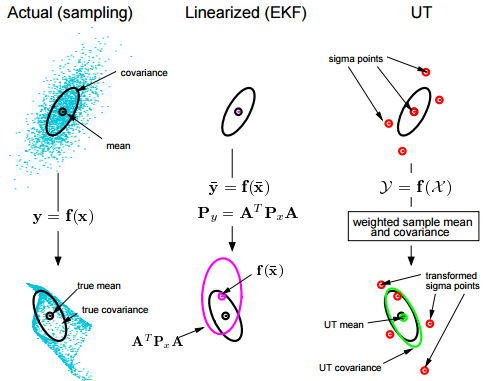
\includegraphics[width=0.8\textwidth]{figures/datared/StateTransformation.png}
    \caption{Propagation of states $\mathbf{x}$ through a non linear function $\mathbf{f}$ for different transformation techniques.
    The left plot shows the true mean and covariance propagation which uses Monte-Carlo sampling.
    The middle shows the linearisation performed by the extended Kalman filter (EKF), another non-linear Kalman filter.
    The right plot shows the propagation performed with the unscented transform used by the UKF.
    The performace of the UKF is superior to that of the EKF and uses much less sampling points (called sigma points) than Monte-Carlo samping.}
    \label{fig:State propagation for different filters}
\end{figure}

\subsection{Summary of hidden Markov model formulation}
\label{sub:Summary of hidden Markov model formulation}
In summary the diffraction experiment has been represented as a hidden Markov model where a process function describes how the (hidden) state of the crystal at a particular time point i generates the consecutive crystal state due to X-ray irradiation.
An observation model also describes how the crystal, which is in a particular state, generates the observed intensities.
The UKF and the URTSS algorithms together give the forward-backward algorithm, which is designed to give the optimal sequence of crystal states that best describe the observed data that is consistent with the defined process and observation functions.
The process and observation (co)variances quantify the level of uncertainty of the corresponding processes.
The forward-backward algorithm is applied iteratively to obtain the improved estimates of the structure factor amplitude of a reflection with each iteration.
The log likelihood is calculated for each cycle and when the improvement of the log likelihood is smaller than a given tolerance value, the solution is considered to have converged.
The final result of the algorithm is a sequence of the set of structure factor amplitudes for each time point in the data collection experiment.
